% ============================================================
\chapter{Classical Thermodynamics}
% ============================================================

% ============================================================
\section{Thermal Equilibrium and Temperature}
% ============================================================

\begin{definition}[Temperature]
Temperature is the quantity equal for two objects in \emph{thermal equilibrium}. It measures the tendency to give up energy: a hotter object transfers energy to a cooler one until their temperatures equalize.
\end{definition}

\begin{definition}[Relaxation time]
The \textbf{relaxation time} is the characteristic time to reach thermal equilibrium. It varies enormously --- from femtoseconds in dense plasmas to geological timescales in some solids.
\end{definition}

Beyond thermal equilibrium, a system may reach \textbf{mechanical equilibrium} (no net forces or pressure gradients) and \textbf{diffusive equilibrium} (equal chemical potentials, no net particle flow). All three together constitute \emph{thermodynamic equilibrium}.

\begin{fact}[Zeroth Law of Thermodynamics]
If $A$ is in thermal equilibrium with $C$, and $B$ is also in thermal equilibrium with $C$, then $A$ and $B$ are in thermal equilibrium with each other. This transitivity makes temperature a well-defined, measurable quantity.
\end{fact}

% ============================================================
\section{The Ideal Gas}
% ============================================================

\subsection{Kinetic Derivation of the Ideal Gas Law}

\begin{example}
We derive the ideal gas law for $N$ point particles bouncing elastically inside a box of side $L$ and volume $V = L^3$.

\begin{center}
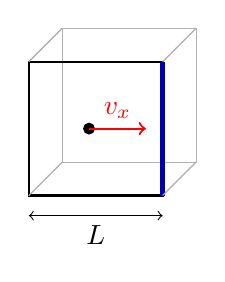
\begin{tikzpicture}[scale=0.85]
  % Back face of box
  \draw[gray!60] (0.5,0.5) -- (2.5,0.5) -- (2.5,2.5) -- (0.5,2.5) -- cycle;
  \draw[gray!60] (0.5,0.5) -- (0,0);
  \draw[gray!60] (2.5,0.5) -- (2,0);
  \draw[gray!60] (2.5,2.5) -- (2,2);
  \draw[gray!60] (0.5,2.5) -- (0,2);
  % Front face of box
  \draw[thick] (0,0) -- (2,0) -- (2,2) -- (0,2) -- cycle;
  % Right wall highlighted
  \draw[thick, blue!70!black, line width=2pt] (2,0) -- (2,2);
  % Depth edges
  \draw[gray!60] (0,0) -- (0.5,0.5);
  \draw[gray!60] (2,0) -- (2.5,0.5);
  \draw[gray!60] (2,2) -- (2.5,2.5);
  \draw[gray!60] (0,2) -- (0.5,2.5);
  % Particle
  \filldraw[black] (0.9,1.0) circle (0.08);
  % Velocity arrow
  \draw[->, thick, red] (0.9,1.0) -- (1.75,1.0) node[midway, above] {$v_x$};
  % Side length label
  \draw[<->] (0,-0.3) -- (2,-0.3) node[midway, below] {$L$};
\end{tikzpicture}\\[3pt]
{\small\itshape Particle with velocity $v_x$ bouncing elastically off the right wall of a box of side $L$.}
\end{center}

Elastic reflection reverses only the normal component, so the momentum transferred per collision is $\Delta p_{xi} = 2mv_{xi}$. The round-trip time is $\Delta t = 2L/v_{xi}$, giving a time-averaged force from particle $i$:
\begin{equation}
    F_{xi} = \frac{\Delta p_{xi}}{\Delta t} = \frac{mv_{xi}^2}{L}.
\end{equation}
Summing over all $N$ particles and using isotropy $\langle v_x^2\rangle = \langle v_y^2\rangle = \langle v_z^2\rangle \equiv \tfrac{1}{3}\langle v^2\rangle$, the pressure $P = F_x/L^2$ is
\begin{equation}
    P = \frac{mN\langle v^2\rangle}{3V}.
\end{equation}
Setting $k_BT \equiv \tfrac{1}{3}m\langle v^2\rangle$ (consistent with the equipartition theorem, Section~\ref{sec:equipartition}):

\begin{formula}[Ideal Gas Law]
\begin{equation}
    PV = Nk_BT \qquad \text{or equivalently} \qquad PV = nRT,
\end{equation}
where $n$ is the number of moles, $R = 8.31\,\mathrm{J\,mol^{-1}\,K^{-1}}$, and $k_B = R/N_A = 1.38\times10^{-23}\,\mathrm{J/K}$.
\end{formula}

The mean internal energy is $\langle U\rangle = \tfrac{3}{2}Nk_BT$, purely kinetic, extensive in $N$.
\end{example}

\begin{center}
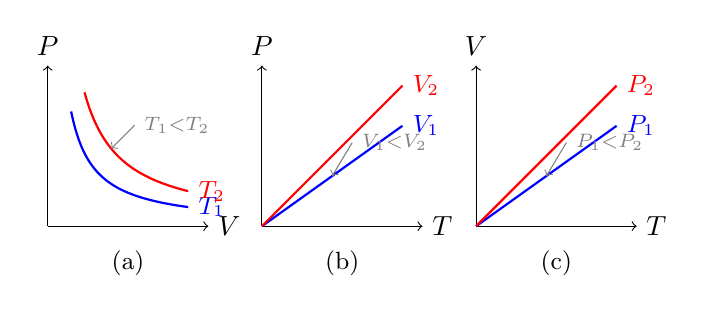
\begin{tikzpicture}[scale=0.85]
  % Panel (a): P vs V isotherms
  \begin{scope}[xshift=0cm]
    \draw[->] (0,0) -- (2.4,0) node[right] {$V$};
    \draw[->] (0,0) -- (0,2.4) node[above] {$P$};
    \draw[blue,  domain=0.35:2.1, samples=60, thick] plot (\x, {0.6/\x}) node[right,font=\small] {$T_1$};
    \draw[red,   domain=0.55:2.1, samples=60, thick] plot (\x, {1.1/\x}) node[right,font=\small] {$T_2$};
    \node[font=\small] at (1.2,-0.55) {(a)};
    \node[font=\scriptsize, blue] at (1.9,0.55) {};
    \draw[<-,gray,font=\scriptsize] (0.95,1.16) -- ++(0.35,0.35) node[right,font=\scriptsize] {$T_1{<}T_2$};
  \end{scope}
  % Panel (b): P vs T isochores
  \begin{scope}[xshift=3.2cm]
    \draw[->] (0,0) -- (2.4,0) node[right] {$T$};
    \draw[->] (0,0) -- (0,2.4) node[above] {$P$};
    \draw[blue,  thick] (0,0) -- (2.1,1.5) node[right,font=\small] {$V_1$};
    \draw[red,   thick] (0,0) -- (2.1,2.1) node[right,font=\small] {$V_2$};
    \draw[<-,gray] (1.05,0.75) -- ++(0.3,0.5) node[right,font=\scriptsize] {$V_1{<}V_2$};
    \node[font=\small] at (1.2,-0.55) {(b)};
  \end{scope}
  % Panel (c): V vs T isobars
  \begin{scope}[xshift=6.4cm]
    \draw[->] (0,0) -- (2.4,0) node[right] {$T$};
    \draw[->] (0,0) -- (0,2.4) node[above] {$V$};
    \draw[blue,  thick] (0,0) -- (2.1,1.5) node[right,font=\small] {$P_1$};
    \draw[red,   thick] (0,0) -- (2.1,2.1) node[right,font=\small] {$P_2$};
    \draw[<-,gray] (1.05,0.75) -- ++(0.3,0.5) node[right,font=\scriptsize] {$P_1{<}P_2$};
    \node[font=\small] at (1.2,-0.55) {(c)};
  \end{scope}
\end{tikzpicture}\\[3pt]
{\small\itshape Ideal gas: (a) isotherms in $P$--$V$, (b) isochores in $P$--$T$, (c) isobars in $V$--$T$.}
\end{center}

\subsection{The Barometric Formula}

\begin{example}
Consider a thin atmospheric slab at height $z$, thickness $dz$, area $A$. Vertical force balance gives $dP/dz = -\rho g$. Using $\rho = mP/(k_BT)$:

\begin{center}
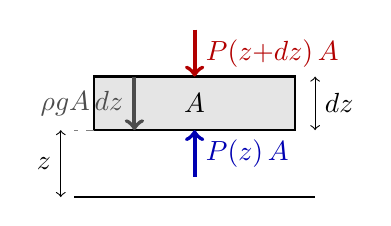
\begin{tikzpicture}[scale=0.85]
  % Slab rectangle
  \fill[gray!20] (0,1.0) rectangle (3.0,1.8);
  \draw[thick] (0,1.0) rectangle (3.0,1.8);
  % Area label
  \node at (1.5,1.4) {$A$};
  % Thickness label
  \draw[<->] (3.3,1.0) -- (3.3,1.8) node[midway, right] {$dz$};
  % Height label
  \draw[<->] (-0.5,0) -- (-0.5,1.0) node[midway, left] {$z$};
  \draw[dashed, gray] (0,0) -- (-0.3,0);
  \draw[dashed, gray] (0,1.0) -- (-0.3,1.0);
  % Ground line
  \draw[thick] (-0.3,0) -- (3.3,0);
  % P(z) arrow upward from below
  \draw[->, thick, blue!70!black, line width=1.5pt] (1.5,0.3) -- (1.5,1.0)
    node[midway, right] {$P(z)\,A$};
  % P(z+dz) arrow downward from above
  \draw[->, thick, red!70!black, line width=1.5pt] (1.5,2.5) -- (1.5,1.8)
    node[midway, right] {$P(z{+}dz)\,A$};
  % Weight arrow
  \draw[->, thick, black!70, line width=1.5pt] (0.6,1.8) -- (0.6,1.0)
    node[midway, left] {$\rho g A\,dz$};
\end{tikzpicture}\\[3pt]
{\small\itshape Force balance on an atmospheric slab of area $A$ and thickness $dz$ at height $z$.}
\end{center}

\begin{equation}
    \dv{P}{z} = -\frac{mg}{k_BT}\,P.
\end{equation}
At constant $T$ this integrates to the

\begin{formula}[Barometric Formula]
\begin{equation}
    P(z) = P(0)\,e^{-mgz/(k_BT)}.
\end{equation}
\end{formula}

Pressure falls exponentially with scale height $H = k_BT/(mg)$. For air ($\bar{M} \approx 29\,\mathrm{g/mol}$, $T = 300\,\mathrm{K}$), $H \approx 8.5\,\mathrm{km}$.
\end{example}

% ============================================================
\section{The Van der Waals Gas}
% ============================================================

Real gases deviate from the ideal gas law due to finite molecular size (short-range repulsion) and attractive interactions at larger separations. The Van der Waals model captures both with two parameters $a$ and $b$.

\begin{center}
\begin{tikzpicture}[scale=0.85]
  \draw[->] (0,-1.6) -- (0,2.8) node[above] {$V(r)$};
  \draw[->] (0,0) -- (5.2,0) node[right] {$r$};
  % Lennard-Jones-like curve: repulsive wall, well near r=R, approaches 0
  \draw[thick, blue!80!black, domain=0.72:4.8, samples=120]
    plot (\x, { 0.8/(\x-0.5)^2 - 1.2/(\x+0.1) + 0.18 });
  % Zero dashed line
  \draw[dashed, gray] (0,0) -- (5.0,0);
  % Mark well minimum near r=R (approximately x=1.4)
  \draw[dashed, gray] (1.55,-1.25) -- (1.55,0);
  \node[below] at (1.55,0) {$R$};
  % Well depth annotation
  \draw[<->] (2.4,-1.25) -- (2.4,0) node[midway, right] {\small well depth};
  \draw[dashed, gray] (1.55,-1.25) -- (2.4,-1.25);
  % Label approaching zero
  \node[right, font=\small] at (4.2,0.15) {$V\to 0$};
\end{tikzpicture}\\[3pt]
{\small\itshape Lennard-Jones-type intermolecular potential: hard-core repulsion at short range, attractive well near $r=R$.}
\end{center}

\textbf{Excluded volume.} Each molecule excludes others from a volume $b$, reducing the available volume from $V$ to $V - Nb$.

\textbf{Attractive interactions.} A molecule near the wall is pulled inward. The cohesive pressure correction scales as $(N/V)^2$, reducing effective pressure by $aN^2/V^2$.

Substituting both corrections ($V \to V-Nb$, $P \to P + aN^2/V^2$) into the ideal gas law:

\begin{formula}[Van der Waals Equation of State]
\begin{equation}
    \left(P + \frac{aN^2}{V^2}\right)(V - Nb) = Nk_BT.
\end{equation}
\end{formula}

In the dilute limit $Nb \ll V$ and $aN^2/V^2 \ll P$, this reduces to the ideal gas law.

% ============================================================
\section{The Equipartition Theorem}
\label{sec:equipartition}
% ============================================================

\begin{theorem}[Equipartition Theorem]
In classical thermal equilibrium at temperature $T$, the mean of any energy term quadratic in a coordinate or momentum is $\tfrac{1}{2}k_BT$:
\begin{equation}
    \left\langle\tfrac{1}{2}\alpha q^2\right\rangle = \tfrac{1}{2}k_BT.
\end{equation}
\end{theorem}

This applies to translational kinetic energies $\tfrac{1}{2}mv_x^2$, $\tfrac{1}{2}mv_y^2$, $\tfrac{1}{2}mv_z^2$; rotational energies $\tfrac{1}{2}I\omega^2$; and both the kinetic $\tfrac{1}{2}\mu\dot{r}^2$ and potential $\tfrac{1}{2}kr^2$ terms of a vibrational mode.

\textbf{Counting degrees of freedom.} A monatomic ideal gas has $f = 3$ translational DOF. A diatomic molecule has 3 translational + 2 rotational (the bond-axis rotation is quantum mechanically frozen) + 2 vibrational = $f = 7$ classically; in practice $f = 5$ at room temperature since vibrational modes are not thermally activated.

\begin{center}
\begin{tikzpicture}[scale=0.85]
  % === Left: Dumbbell with rotational arrows ===
  % Bond axis (horizontal)
  \draw[thick] (0,0) -- (2.0,0);
  % Atoms
  \filldraw[gray!40, draw=black, thick] (0,0) circle (0.28);
  \filldraw[gray!40, draw=black, thick] (2.0,0) circle (0.28);
  % Rotation arrow 1 (perpendicular: in the plane, curving around vertical axis through center)
  \draw[->, thick, blue!70!black] (1.0, 0.4) arc (90:350:0.42 and 0.35)
    node[above right, font=\small] {};
  % Rotation arrow 2 (out of plane: dashed arc)
  \draw[->, thick, red!70!black, dashed] (1.0,-0.05) ellipse (0.42 and 0.20);
  \node[font=\small] at (1.0,-0.85) {rotation};

  % === Right: Spring model ===
  \begin{scope}[xshift=4.5cm]
    % Left mass
    \filldraw[gray!40, draw=black, thick] (0,0) circle (0.28);
    % Spring (zigzag)
    \draw[thick, decorate, decoration={coil, segment length=4pt, amplitude=4pt}]
      (0.28,0) -- (1.72,0);
    % Right mass
    \filldraw[gray!40, draw=black, thick] (2.0,0) circle (0.28);
    % Labels
    \node[font=\small, below] at (1.0,-0.35) {$\tfrac{1}{2}\mu\dot{r}^2 + \tfrac{1}{2}kr^2$};
    \node[font=\small] at (1.0,-0.85) {vibration};
  \end{scope}

  % Dividing line
  \draw[gray, dashed] (3.5,-1.2) -- (3.5,1.0);
\end{tikzpicture}\\[3pt]
{\small\itshape Diatomic molecule: two rotational DOF perpendicular to bond axis (left); spring model for vibration (right).}
\end{center}

A mode is frozen out when $k_BT \ll \hbar\omega$, so $f$ rises with temperature. Measured heat capacities of diatomic gases transition from $f=3$ at very low $T$, through $f=5$ at room temperature, toward $f=7$ at high $T$.

\begin{formula}
\begin{equation}
    U_{\text{thermal}} = \frac{f}{2}Nk_BT.
\end{equation}
\end{formula}

Differentiating gives $C_V = \tfrac{f}{2}Nk_B$. For a crystal, each atom has $f=6$ (3 vibrational modes, each with 2 quadratic terms):

\begin{theorem}[Dulong--Petit Law]
\begin{equation}
    U = 3Nk_BT, \qquad C_V = 3Nk_B = 3nR.
\end{equation}
This agrees well with measured room-temperature heat capacities of elemental solids; it fails at low $T$ where quantum mechanics suppresses vibrational modes.
\end{theorem}

% ============================================================
\section{Heat, Work, and the First Law}
% ============================================================

\begin{definition}[Heat and Work]
\textbf{Heat} is energy flow driven by a temperature difference. \textbf{Work} is any other energy transfer. Both are processes, not state properties.
\end{definition}

Heat transfer mechanisms: \textbf{conduction} (direct molecular contact), \textbf{convection} (bulk fluid motion), \textbf{radiation} (electromagnetic emission/absorption, requires no medium).

\begin{center}
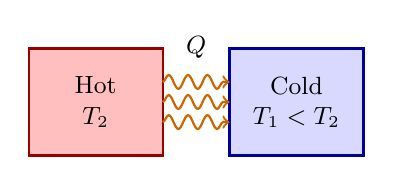
\begin{tikzpicture}[scale=0.85]
  % Hot block
  \fill[red!25] (0,0) rectangle (2.0,1.6);
  \draw[thick, red!60!black] (0,0) rectangle (2.0,1.6);
  \node[font=\small, align=center] at (1.0,0.8) {Hot\\$T_2$};
  % Cold block
  \fill[blue!15] (3.0,0) rectangle (5.0,1.6);
  \draw[thick, blue!60!black] (3.0,0) rectangle (5.0,1.6);
  \node[font=\small, align=center] at (4.0,0.8) {Cold\\$T_1 < T_2$};
  % Wavy arrows from hot to cold
  \draw[->, thick, orange!80!black, decorate,
        decoration={snake, amplitude=2.5pt, segment length=7pt}]
    (2.0,1.1) -- (3.0,1.1);
  \draw[->, thick, orange!80!black, decorate,
        decoration={snake, amplitude=2.5pt, segment length=7pt}]
    (2.0,0.8) -- (3.0,0.8);
  \draw[->, thick, orange!80!black, decorate,
        decoration={snake, amplitude=2.5pt, segment length=7pt}]
    (2.0,0.5) -- (3.0,0.5);
  \node[above, font=\small] at (2.5,1.3) {$Q$};
\end{tikzpicture}\\[3pt]
{\small\itshape Spontaneous heat flow from hot to cold by conduction.}
\end{center}

\begin{theorem}[First Law of Thermodynamics]
For a closed system:
\begin{equation}
    dU = \dbar Q + \dbar W.
\end{equation}
$U$ is a \emph{state function} (exact differential; $\Delta U$ depends only on endpoints). $\dbar Q$ and $\dbar W$ are \emph{inexact} differentials --- their integrals depend on the path, not just the endpoints.
\end{theorem}

\subsection{Compression Work}

\begin{center}
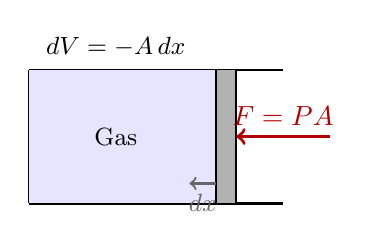
\begin{tikzpicture}[scale=0.85]
  % Cylinder walls (top and bottom)
  \draw[thick] (0,0) -- (3.8,0);
  \draw[thick] (0,2.0) -- (3.8,2.0);
  % Left closed end
  \draw[thick] (0,0) -- (0,2.0);
  % Gas fill
  \fill[blue!10] (0,0) rectangle (2.8,2.0);
  \node[font=\small] at (1.3,1.0) {Gas};
  % Piston (thick vertical line)
  \fill[gray!60] (2.8,0) rectangle (3.1,2.0);
  \draw[thick] (2.8,0) -- (2.8,2.0);
  \draw[thick] (3.1,0) -- (3.1,2.0);
  % Force arrow pointing left
  \draw[->, very thick, red!70!black] (4.5,1.0) -- (3.1,1.0)
    node[midway, above] {$F = PA$};
  % Displacement arrow dx pointing left (smaller, below)
  \draw[<-, thick, black!60] (2.4,0.3) -- (2.8,0.3)
    node[midway, below, font=\small] {$dx$};
  % dV label
  \node[font=\small, above] at (1.3,2.05) {$dV = -A\,dx$};
\end{tikzpicture}\\[3pt]
{\small\itshape Quasistatic compression: piston of area $A$ moves inward by $dx$, reducing volume by $dV=A\,dx$.}
\end{center}

For a \textbf{quasistatic} process (gas in equilibrium throughout), moving the piston inward by $dx$ decreases volume by $dV = -A\,dx$:

\begin{formula}[Compression Work]
\begin{equation}
    W = -\int_{V_i}^{V_f} P(V)\,dV.
\end{equation}
\end{formula}

Compression gives $W > 0$; expansion gives $W < 0$. For non-quasistatic processes, only $\Delta U$ is well-defined.

\subsection{Heat Capacities}

\begin{definition}[Heat Capacity]
$C = Q/\Delta T$; the specific heat capacity is $c = C/m$.
\end{definition}

\textbf{Constant volume.} $dV = 0 \Rightarrow \dbar W = 0$, so $\dbar Q = dU$:

\begin{formula}[Heat Capacity at Constant Volume]
\begin{equation}
    C_V = \left.\pdv{U}{T}\right|_V.
\end{equation}
\end{formula}

For an ideal gas, $C_V = \tfrac{f}{2}Nk_B$.

\textbf{Constant pressure.} From $\dbar Q = dU + P\,dV$:
\begin{equation}
    C_P = \left.\pdv{U}{T}\right|_P + P\left.\pdv{V}{T}\right|_P.
\end{equation}
For an ideal gas, $(\partial U/\partial V)_T = 0$ and $(\partial V/\partial T)_P = Nk_B/P$, giving

\begin{formula}[$C_P$ for an Ideal Gas (Mayer's Relation)]
\begin{equation}
    C_P = C_V + Nk_B = C_V + nR.
\end{equation}
\end{formula}

The extra $Nk_B$ is work done against the surroundings. The adiabatic index is $\gamma = C_P/C_V = (f+2)/f$.

\begin{center}
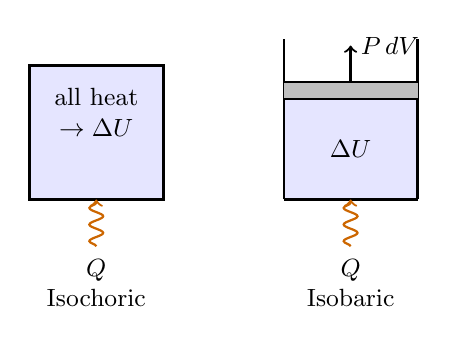
\begin{tikzpicture}[scale=0.85]
  %% Left panel: Isochoric (rigid container)
  \begin{scope}[xshift=0cm]
    % Rigid container
    \fill[blue!10] (0,0) rectangle (2.0,2.0);
    \draw[very thick] (0,0) rectangle (2.0,2.0);
    \node[font=\small, align=center] at (1.0,1.3) {all heat\\$\to \Delta U$};
    % Heat arrow in from below
    \draw[->, thick, orange!80!black, decorate,
          decoration={snake, amplitude=2.5pt, segment length=6pt}]
      (1.0,-0.7) -- (1.0,0.0);
    \node[below, font=\small] at (1.0,-0.75) {$Q$};
    \node[below, font=\small] at (1.0,-1.2) {Isochoric};
  \end{scope}

  %% Right panel: Isobaric (piston-cylinder)
  \begin{scope}[xshift=3.8cm]
    % Cylinder walls and gas
    \fill[blue!10] (0,0) rectangle (2.0,1.5);
    \draw[thick] (0,0) -- (2.0,0);
    \draw[thick] (0,0) -- (0,2.4);
    \draw[thick] (2.0,0) -- (2.0,2.4);
    % Piston
    \fill[gray!50] (0,1.5) rectangle (2.0,1.75);
    \draw[thick] (0,1.5) -- (2.0,1.5);
    \draw[thick] (0,1.75) -- (2.0,1.75);
    % Piston rising arrow
    \draw[->, thick, black] (1.0,1.75) -- (1.0,2.3)
      node[right, font=\small] {$P\,dV$};
    % Internal energy label
    \node[font=\small] at (1.0,0.75) {$\Delta U$};
    % Heat arrow in from below
    \draw[->, thick, orange!80!black, decorate,
          decoration={snake, amplitude=2.5pt, segment length=6pt}]
      (1.0,-0.7) -- (1.0,0.0);
    \node[below, font=\small] at (1.0,-0.75) {$Q$};
    \node[below, font=\small] at (1.0,-1.2) {Isobaric};
  \end{scope}
\end{tikzpicture}\\[3pt]
{\small\itshape Isochoric: all heat becomes internal energy. Isobaric: heat splits between $\Delta U$ and $P\,dV$ work.}
\end{center}

\subsection{Latent Heat}

During a phase transition, heat is absorbed at constant temperature ($C \to \infty$).

\begin{definition}[Latent Heat]
The specific latent heat $\ell = L/m$ ($\mathrm{J/kg}$) is the heat per unit mass for a phase change at constant $P$. The absorbed energy breaks bonds rather than increasing kinetic energy. Values: melting ice $333\,\mathrm{J/g}$; boiling water $2260\,\mathrm{J/g}$.
\end{definition}

% ============================================================
\section{Thermodynamic Processes}
% ============================================================

A quasi-static transformation traces a definite path in state space. $\Delta U = U_f - U_i$ is path-independent; $W$ and $Q$ are obtained by integrating along the path.

\subsection{Isothermal Compression}

At constant $T$: $PV = Nk_BT = \text{const}$, so

\begin{formula}[Isothermal Work, Ideal Gas]
\begin{equation}
    W = -\int_{V_i}^{V_f}\frac{Nk_BT}{V}\,dV = Nk_BT\ln\frac{V_i}{V_f}.
\end{equation}
\end{formula}

Since $\Delta U = 0$, the First Law gives $Q = -W$: all work done flows out as heat to the reservoir.

\subsection{Adiabatic Compression}

No heat exchange: $\dbar Q = 0$. With $dU = C_V\,dT$ and $\dbar W = -P\,dV$:
\begin{equation}
    \frac{f}{2}Nk_B\,dT = -\frac{Nk_BT}{V}\,dV
    \qquad\Longrightarrow\qquad
    \frac{f}{2}\frac{dT}{T} = -\frac{dV}{V}.
\end{equation}
Integrating:

\begin{formula}[Adiabatic Constraints]
\begin{equation}
    VT^{f/2} = \text{const}, \qquad\qquad PV^{\gamma} = \text{const}, \qquad \gamma = \frac{f+2}{f} = \frac{C_P}{C_V}.
\end{equation}
\end{formula}

Since $\gamma > 1$, the adiabat $P \propto V^{-\gamma}$ is steeper than the isotherm $P \propto V^{-1}$: adiabatic compression raises temperature faster.

\begin{center}
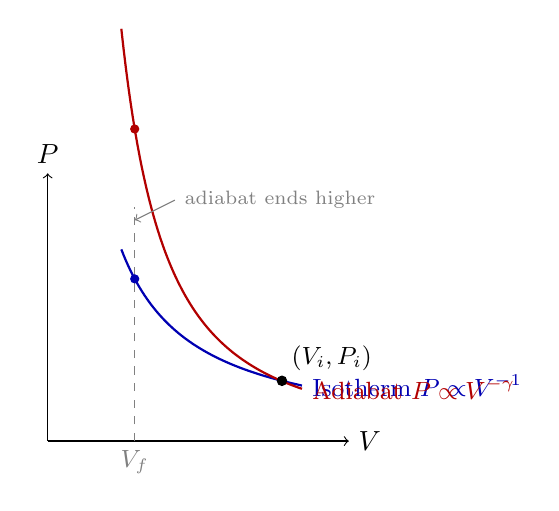
\begin{tikzpicture}[scale=0.85]
  \draw[->] (0,0) -- (4.5,0) node[right] {$V$};
  \draw[->] (0,0) -- (0,4.0) node[above] {$P$};
  % Initial point at (Vi, Pi) = (3.5, 0.9)
  % Final volume Vf = 1.3
  % Isotherm: P*V = const => P = 3.15/V  (passes through (3.5,0.9))
  \draw[thick, blue!70!black, domain=1.1:3.8, samples=80]
    plot (\x, {3.15/\x}) node[right, font=\small] {Isotherm $P\propto V^{-1}$};
  % Adiabat: P*V^gamma = const, gamma=5/3 => P = 3.15 * 3.5^(2/3) / V^(5/3)
  % At V=3.5: P=0.9 (same start). Constant = 0.9*3.5^(5/3) = 0.9*8.02 = 7.22
  \draw[thick, red!70!black, domain=1.1:3.8, samples=80]
    plot (\x, {7.22/(\x^1.667)}) node[right, font=\small] {Adiabat $P\propto V^{-\gamma}$};
  % Mark initial point
  \filldraw (3.5,0.9) circle (0.07) node[above right, font=\small] {$(V_i,P_i)$};
  % Mark Vf dashed line
  \draw[dashed, gray] (1.3,0) node[below, font=\small] {$V_f$} -- (1.3,3.5);
  % Mark endpoints at Vf
  \filldraw[blue!70!black] (1.3, {3.15/1.3}) circle (0.06);
  \filldraw[red!70!black]  (1.3, {7.22/1.3^1.667}) circle (0.06);
  % Annotate that adiabat is higher
  \draw[<-, gray, font=\scriptsize] (1.3,3.3) -- ++(0.6,0.3)
    node[right, font=\scriptsize] {adiabat ends higher};
\end{tikzpicture}\\[3pt]
{\small\itshape Adiabat (steep) vs.\ isotherm (shallow) in the $P$--$V$ plane: adiabatic compression raises temperature more.}
\end{center}

The work done on the gas equals $\Delta U$ (since $Q=0$):
\begin{equation}
    W_{\text{adiabat}} = \Delta U = \frac{f}{2}Nk_B(T_f - T_i)
    = \frac{Nk_BT_i}{\gamma - 1}\!\left[\!\left(\frac{V_f}{V_i}\right)^{1-\gamma} - 1\right].
\end{equation}

\subsection{Isochoric and Isobaric Processes}

\textbf{Isochoric} ($dV = 0$): no work done; $\Delta U = \int C_V\,dT$.

\textbf{Isobaric} (constant $P$): work $\Delta W = -P\Delta V$; heat $\Delta Q = \int C_P\,dT$. On a $P$--$V$ diagram, the isobar is horizontal; the area below gives the work done by the gas.

% ============================================================
\section{Enthalpy}
% ============================================================

\begin{definition}[Enthalpy]
\begin{equation}
    H \coloneq U + PV.
\end{equation}
$H$ is the total energy to create the system: internal energy $U$ plus work $PV$ done against the atmosphere.
\end{definition}

\begin{center}
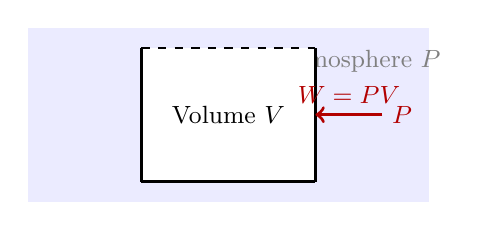
\begin{tikzpicture}[scale=0.85]
  % Atmosphere region (background)
  \fill[blue!8] (-0.5,-0.3) rectangle (5.5,2.3);
  \node[font=\small, gray] at (4.5,1.8) {atmosphere $P$};
  % Container (open box: left, bottom, right walls)
  \fill[white] (1.2,0) rectangle (3.8,2.0);
  \draw[very thick] (1.2,0) -- (1.2,2.0);
  \draw[very thick] (1.2,0) -- (3.8,0);
  \draw[very thick] (3.8,0) -- (3.8,2.0);
  % Dashed top (open top or being pushed in)
  \draw[dashed, thick] (1.2,2.0) -- (3.8,2.0);
  % Volume label inside
  \node[font=\small] at (2.5,1.0) {Volume $V$};
  % Arrow showing atmosphere pressing (from right)
  \draw[->, very thick, red!70!black] (4.8,1.0) -- (3.8,1.0)
    node[midway, above, font=\small] {$W = PV$};
  \node[right, font=\small, red!70!black] at (4.8,1.0) {$P$};
\end{tikzpicture}\\[3pt]
{\small\itshape Enthalpy includes the work $PV$ done against atmosphere to make room for the system.}
\end{center}

\subsection{Why Enthalpy is Convenient}

Differentiating $H = U + PV$ and using $dU = \dbar Q - P\,dV + \dbar W_{\text{other}}$:
\begin{equation}
    dH = \dbar Q + V\,dP + \dbar W_{\text{other}}.
\end{equation}
At constant $P$ with no other work:

\begin{formula}
\begin{equation}
    \Delta H = Q \qquad (\text{constant pressure, no other work}).
\end{equation}
\end{formula}

More generally, $\Delta H = Q + W_{\text{other}}$.

\subsection{Heat Capacity at Constant Pressure}

Since $dH = \dbar Q$ at constant $P$:

\begin{formula}
\begin{equation}
    C_P = \left.\pdv{H}{T}\right|_P.
\end{equation}
\end{formula}


\subsection{Enthalpy of Formation}

\begin{example}
Standard enthalpy tables give the heat released or absorbed forming compounds from elements at $1\,\mathrm{atm}$, $298\,\mathrm{K}$. For liquid water:
\begin{equation}
    \mathrm{H_2} + \tfrac{1}{2}\,\mathrm{O_2} \longrightarrow \mathrm{H_2O}\,(\ell), \qquad \Delta H = -286\,\mathrm{kJ/mol}.
\end{equation}
Boiling water at $373\,\mathrm{K}$, $1\,\mathrm{atm}$: $\Delta H = 40{,}660\,\mathrm{J/mol}$, of which $PV = RT \approx 3100\,\mathrm{J/mol}$ is $pV$ work.
\end{example}

% ============================================================
\section{Rates of Processes}
% ============================================================

\subsection{Heat Conduction and Fourier's Law}


\begin{center}
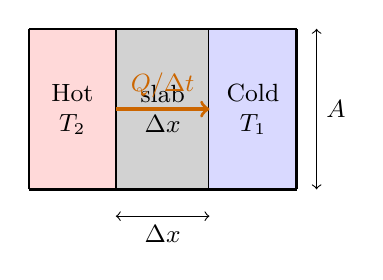
\begin{tikzpicture}[scale=0.85]
  % Hot side (left)
  \fill[red!15] (0,0) rectangle (1.3,2.4);
  \node[font=\small, align=center] at (0.65,1.2) {Hot\\$T_2$};
  % Slab (wall)
  \fill[gray!35] (1.3,0) rectangle (2.7,2.4);
  \draw[thick] (1.3,0) rectangle (2.7,2.4);
  \node[font=\small, align=center] at (2.0,1.2) {slab\\$\Delta x$};
  % Cold side (right)
  \fill[blue!15] (2.7,0) rectangle (4.0,2.4);
  \node[font=\small, align=center] at (3.35,1.2) {Cold\\$T_1$};
  % Boundary lines
  \draw[thick] (0,0) -- (0,2.4);
  \draw[thick] (0,0) -- (4.0,0);
  \draw[thick] (0,2.4) -- (4.0,2.4);
  \draw[thick] (4.0,0) -- (4.0,2.4);
  % Thickness label
  \draw[<->] (1.3,-0.4) -- (2.7,-0.4) node[midway, below, font=\small] {$\Delta x$};
  % Area label
  \draw[<->] (4.3,0) -- (4.3,2.4) node[midway, right, font=\small] {$A$};
  % Heat flow arrow
  \draw[->, very thick, orange!80!black] (1.3,1.2) -- (2.7,1.2)
    node[midway, above, font=\small] {$Q/\Delta t$};
\end{tikzpicture}\\[3pt]
{\small\itshape Fourier's law: heat flux through a slab of thickness $\Delta x$ is proportional to the temperature gradient.}
\end{center}

\begin{formula}[Fourier's Law of Heat Conduction]
\begin{equation}
    \frac{Q}{\Delta t} = -k_t\,A\,\frac{\partial T}{\partial x},
\end{equation}
where $k_t$ is the \textbf{thermal conductivity}. The negative sign ensures flow toward lower temperature.
\end{formula}

Thermal conductivities (in $\mathrm{W\,m^{-1}K^{-1}}$): air ($0.026$), wood ($0.08$), water ($0.6$), glass ($0.8$), iron ($80$), copper ($400$). Metals conduct well because free electrons dominate transport over lattice phonons.

\subsection{Thermal Conductivity from Kinetic Theory}

The key scale is the \textbf{mean free path} $\ell$. For spheres of radius $r$, a collision requires centres within $2r$; setting the swept cylinder volume equal to the volume per molecule:
\begin{equation}
    \ell \approx \frac{1}{4\pi r^2}\cdot\frac{V}{N}.
\end{equation}

\begin{center}
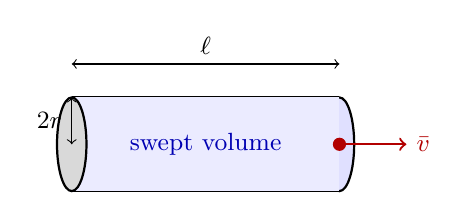
\begin{tikzpicture}[scale=0.85]
  % Draw the cylinder (shown as an ellipse + rectangle for 3D effect)
  % Cylinder axis is horizontal, radius 2r, length ell
  % Front ellipse at right end
  \fill[blue!12] (4.5,1.0) ellipse (0.22 and 0.7);
  \draw[thick] (4.5,1.0) ellipse (0.22 and 0.7);
  % Top and bottom edges of cylinder
  \draw[thick] (0.5, 1.7) -- (4.5, 1.7);
  \draw[thick] (0.5, 0.3) -- (4.5, 0.3);
  % Fill interior
  \fill[blue!8] (0.5,0.3) rectangle (4.5,1.7);
  \draw[dashed, blue!60] (0.5,1.0) ellipse (0.22 and 0.7);
  % Cross-section circle at left (the collision cross section)
  \fill[gray!30] (0.5,1.0) ellipse (0.22 and 0.7);
  \draw[thick] (0.5,1.0) ellipse (0.22 and 0.7);
  % Label 2r on the cross section
  \draw[<->] (0.5,1.0) -- (0.5,1.7) node[midway, left, font=\small] {$2r$};
  % Length label
  \draw[<->] (0.5,2.2) -- (4.5,2.2) node[midway, above, font=\small] {$\ell$};
  % Moving molecule (dot at right face center)
  \filldraw[red!70!black] (4.5,1.0) circle (0.09);
  % Velocity arrow
  \draw[->, thick, red!70!black] (4.5,1.0) -- (5.5,1.0) node[right, font=\small] {$\bar{v}$};
  % Label swept volume
  \node[font=\small, blue!70!black] at (2.5,1.0) {swept volume};
\end{tikzpicture}\\[3pt]
{\small\itshape Mean free path $\ell$: the cylinder of radius $2r$ swept before a collision becomes likely.}
\end{center}

In one mean-free-time $\overline{\Delta t} = \ell/\bar{v}$, roughly half the molecules in each slab cross the barrier. Net heat transferred:
\begin{equation}
    Q \approx -\tfrac{1}{2}\,C_V\,(T_2 - T_1) = -\tfrac{1}{2}\,C_V\,\ell\,\frac{\partial T}{\partial x}.
\end{equation}
Comparing with Fourier's law and using $C_V/V = \tfrac{f}{2}P/T$:

\begin{formula}[Thermal Conductivity, Kinetic Theory]
\begin{equation}
    k_t = \frac{1}{2}\,\frac{C_V}{V}\,\bar{v}\,\ell = \frac{f}{4}\,\frac{P}{T}\,\bar{v}\,\ell.
\end{equation}
\end{formula}

Since $\bar{v} \propto T^{1/2}$ and $\ell \propto T/P$: $k_t \propto T^{1/2}$, independent of pressure.

\subsection{Diffusion and Fick's Laws}

\textbf{Diffusion} transports particles down a number density gradient $n$; $J_x$ is the flux (particles per unit area per unit time).

\begin{center}
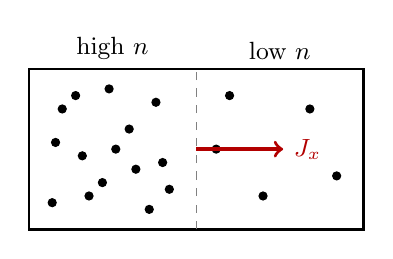
\begin{tikzpicture}[scale=0.85]
  % Outer box
  \draw[thick] (0,0) rectangle (5.0,2.4);
  % Dividing line
  \draw[dashed, gray] (2.5,0) -- (2.5,2.4);
  % Left half label (high concentration) with dots
  \node[font=\small, above] at (1.25,2.4) {high $n$};
  % Many dots on left
  \foreach \x/\y in {0.35/0.4, 0.8/1.1, 0.5/1.8, 1.1/0.7, 1.5/1.5,
                      0.7/2.0, 1.2/2.1, 1.8/0.3, 2.0/1.0, 1.9/1.9,
                      0.4/1.3, 1.6/0.9, 0.9/0.5, 1.3/1.2, 2.1/0.6}{
    \filldraw[black] (\x,\y) circle (0.06);
  }
  % Right half label (low concentration) with fewer dots
  \node[font=\small, above] at (3.75,2.4) {low $n$};
  % Fewer dots on right
  \foreach \x/\y in {2.8/1.2, 3.5/0.5, 4.2/1.8, 3.0/2.0, 4.6/0.8}{
    \filldraw[black] (\x,\y) circle (0.06);
  }
  % Net flux arrow
  \draw[->, very thick, red!70!black] (2.5,1.2) -- (3.8,1.2)
    node[right, font=\small] {$J_x$};
\end{tikzpicture}\\[3pt]
{\small\itshape Diffusion: net particle flux $J_x$ flows down the concentration gradient.}
\end{center}

\begin{formula}[Fick's First Law]
\begin{equation}
    J_x = -D\,\frac{\partial n}{\partial x},
\end{equation}
where $D$ is the \textbf{diffusion coefficient}.
\end{formula}

Combining with particle conservation ($\partial n/\partial t = -\partial J_x/\partial x$):

\begin{formula}[Fick's Second Law]
\begin{equation}
    \frac{\partial n}{\partial t} = D\,\frac{\partial^2 n}{\partial x^2}.
\end{equation}
\end{formula}

A sharp profile spreads with width $\sim\sqrt{Dt}$. By the same kinetic argument:
\begin{equation}
    D \sim \bar{v}\,\ell,
\end{equation}
so the same mean free path governs both energy and particle transport.
